\documentclass[margin=0mm]{standalone}
\usepackage{tikz}
\usepackage{pgfplots}
 \pgfplotsset{compat=newest}




\begin{document}

\pgfmathdeclarefunction{weight_p}{1}{%
  \pgfmathparse{ (#1 -1)/ (2 * 0.1) + sqrt(   (#1 -1)^2/ (2 * 0.1)^2   + 1    ) }%
}
\pgfmathdeclarefunction{weight_m}{1}{%
  \pgfmathparse{ (#1 -1)/ (2 * 0.1) - sqrt(   (#1 -1)^2/ (2 * 0.1)^2   + 1    ) }%
}


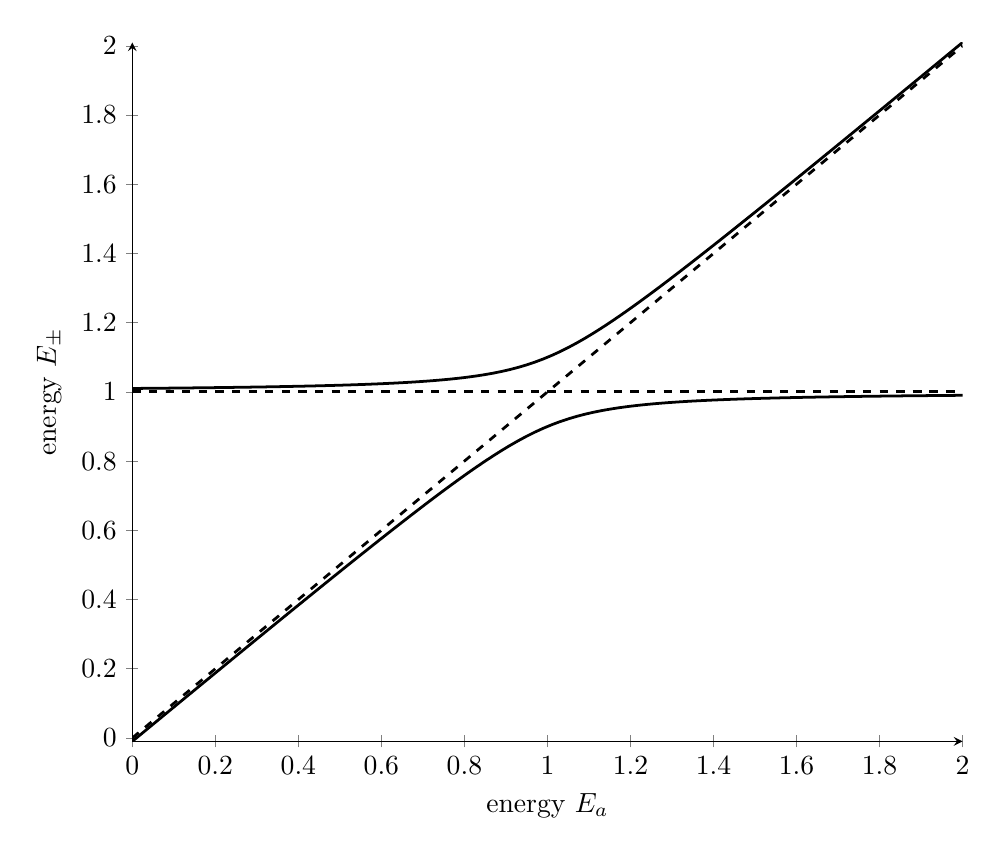
\begin{tikzpicture}
\begin{axis}[no markers, 
        domain=0:2, samples = 100,
          axis y line=left,
           axis x line=bottom,
                      xlabel = {energy $E_a$},
ylabel = {energy $E_\pm$},
           width= \textwidth]
           
\addplot [dashed, line width=1pt]    {x};
\addplot [dashed, line width=1pt]    {1};
\addplot [ line width=1pt]    { (x+1)/2 + sqrt( (x-1)^2 / 4 + 0.1^2) };
\addplot [ line width=1pt]    { (x+1)/2 - sqrt( (x-1)^2 / 4 + 0.1^2) };


\end{axis}
\end{tikzpicture}
\begin{tikzpicture}
\begin{axis}[no markers, 
        domain=0:2, samples = 100,
          axis y line=left,
           axis x line=bottom,
           xlabel = {energy $E_a$},
           width= \textwidth]
           
\addplot [ line width=1pt]    { weight_p(x)^2 / (1 + weight_p(x)^2) };
\addplot [ line width=1pt]    { abs(weight_m(x))^2 / (1 + weight_m(x)^2) };

\end{axis}
\end{tikzpicture}

\end{document}